\subsection{Partial association}\label{sec:mospart}

In a three-way table it may be that two variables, say $A$ and $B$, are
associated at some levels of the third variable, $C$, but not at other
levels of $C$. More generally, we may wish to explore whether and how the
association among two (or more) variables in a contingency table varies over
the levels of the remaining variables. The term \glossterm{partial association} refers
to the association among some variables within the levels of the other
variables.

Consider, for example, the model of conditional independence, $A\perp B\given C$
for a three-way table. This model asserts that $A$ and $B$ are independent
within \textit{each} level of $C$. Denote the hypothesis that $A$ and $B$
are independent at level $C(k)$ by $A\perp B\given C(k)$. Then one can show
\citep{Andersen:91} that

\begin{equation}\label{eq:partial1}
G_{A\perp B\given C}^2=\sum_k^K G_{A\perp B\given C(k)}^2
\end{equation}
That is, the overall \GSQ{} for the conditional independence model
with $(I-1)(J-1)K$ \df{} is the
sum of the values for the ordinary association between $A$ and $B$ over the levels of 
$C$ (each with $(I-1)(J-1)$ \df{}).
Thus, 
\begin{seriate}
\item the overall \GSQ{} may be decomposed into portions attributable
to the $AB$ association in the layers of $C$, and
\item the collection of mosaic displays for the dependence of $A$ and $B$
for each of the levels of $C$ provides a natural visualization of this
decomposition.  These provide an analog, for categorical data, of the conditioning plot, or
\glossterm{coplot}, that
\citet{Cleveland:VisData} has shown to be an effective display for
quantitative data.
\end{seriate}
See \citet{Friendly:99b} for further details.

Mosaic displays for partial association are produced using the \IML{}
module \texttt{mospart}, which is called in a \PROC{IML} step as
\begin{listing}
   run mospart(dim, table, vnames, lnames, title, byvar);
\end{listing}
where \texttt{byvars} specifies the variables which are used to
stratify the data.  One mosaic is produced for each combination
of the levels of the \texttt{byvars}.  In addition, the \macro{MOSAIC}
may be used with a \mparm{BY}{MOSAIC} for the same purpose.
The separate plots may be combined into one figure with the \macro{PANELS},
as illustrated in the following example.


\begin{Example}[employ]{Employment status data}
Data from a 1974 Danish study of 1314 employees who had been laid off are given in \tabref{tab:employ} (from \citet[Table 5.12]{Andersen:91}).
The workers are classified by
\begin{seriate}
\item their employment status, on January 1, 1975 (new job or still unemployed)
\item the cause of their layoff (closure, etc. or replacement)
\item the length of their employment at the time of layoff.
\end{seriate}

%%
%% Table employ written by md2tex 16JUL99 11:22
%%
\begin{table}[htb]
 \caption[Employment Status Data]{Employment Status Data. Employment status on Jan. 1, 1975, by cause of layoff and length of
    previous employment at time of layoff for 1314 employees who lost their
    job in Fall 1974 in Denmark. (Andersen, 1991)}\vspace{5pt}
 \label{tab:employ}
 \begin{center}
  \begin{tabular}{|ll|rrrrrr|}
   \hline
{\bfseries\large Employment} & {\bfseries\large Cause of} & \multicolumn{6}{c|}{\bfseries\large Length of Employment}\rule{0in}{2.5ex}\\
{\bfseries\large Status} & {\bfseries\large Layoff} & $<$1 Mo      & 1-3 Mo     & 3-12 Mo    & 1-2 Yr     & 2-5 Yr     & $>$5 Yr      \\
   \hline
NewJob       & Closure    &    8 &   35 &   70 &   62 &   56 &   38 \\
Unemployed   &            &   10 &   42 &   86 &   80 &   67 &   35 \\
[4pt]
NewJob       & Replaced   &   40 &   85 &  181 &   85 &  118 &   56 \\
Unemployed   &            &   24 &   42 &   41 &   16 &   27 &   10 \\
   \hline
  \end{tabular}
 \end{center}
\end{table}


If employment status (variable $A$) is the response, and cause of layoff ($B$)
and length of employment ($C$) are explanatory, the minimal baseline model
is \([A] \,  [BC] \), in which employment status is independent of both
cause and length.
This model fits quite poorly (\(G^2 (11) = 172.27\)).
The residuals, shown in \figref{fig:mosaic141},
indicate that workers who were laid off as a result of a closure
are more likely to be unemployed, regardless of length of time
they were employed.
Workers who were replaced, however, apparently are more likely
to be employed, particularly if they were employed for 3 months or more.
\begin{figure}[htb]
  \centering
  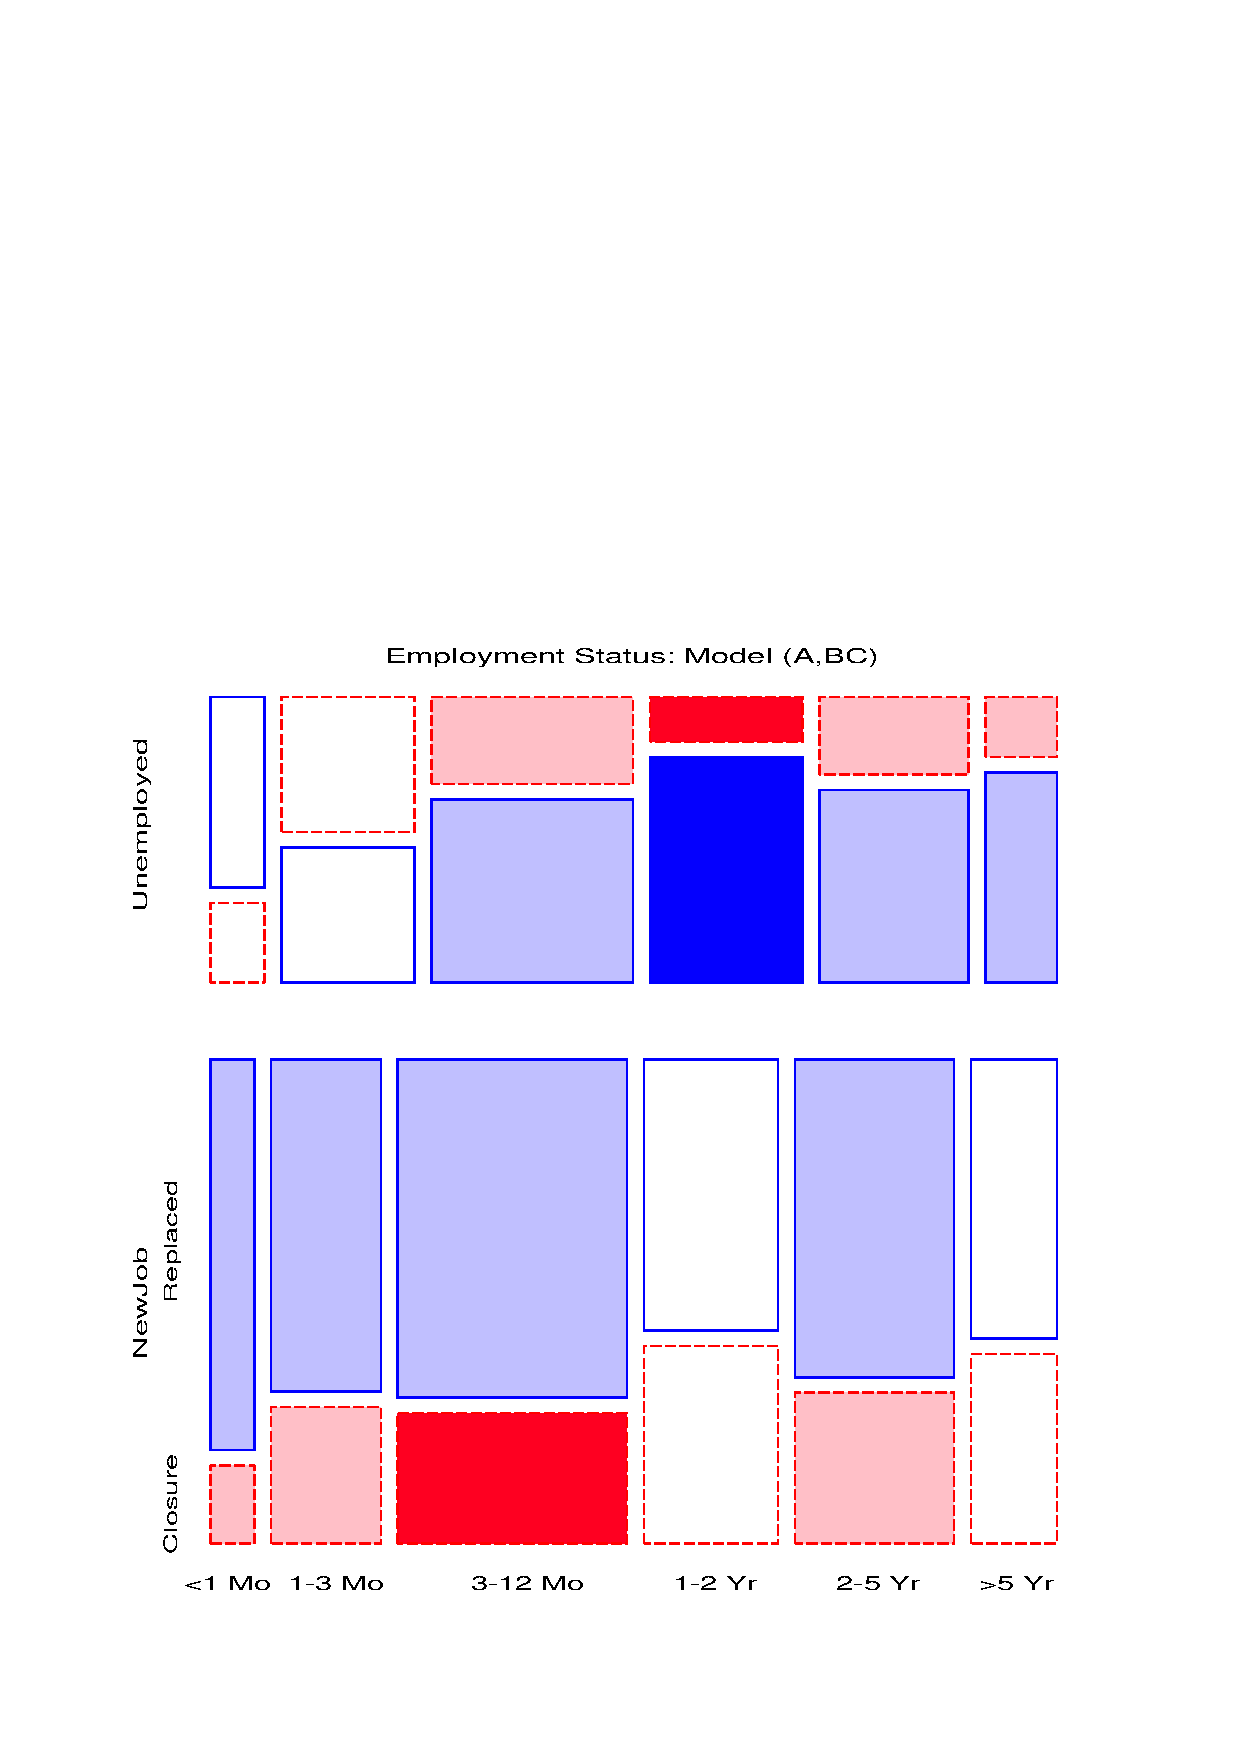
\includegraphics[scale=.6]{ch4/fig/mosaic141}
  \caption[Employment status data, joint independence]{Mosaic display for the employment status data, fitting the model of
joint independence, \([A] \,  [BC] \), \(G^2 (11) = 172.27\)}
  \label{fig:mosaic141} 
\end{figure}

The model of conditional independence, \([AB] \,  [BC] \)
is interpreted as \(A \perp C \given B\);
that is, given the cause of layoff, employment status is independent of length of employment.
This model fits far better (\(G^2 (10) = 24.63\)),
but the lack of fit is still significant.
The residuals, shown in \figref{fig:mosaic143},
suggest that the pattern of association between employment and length
is different for replaced workers and those laid off due to closure.

\begin{figure}[htb]
  \centering
  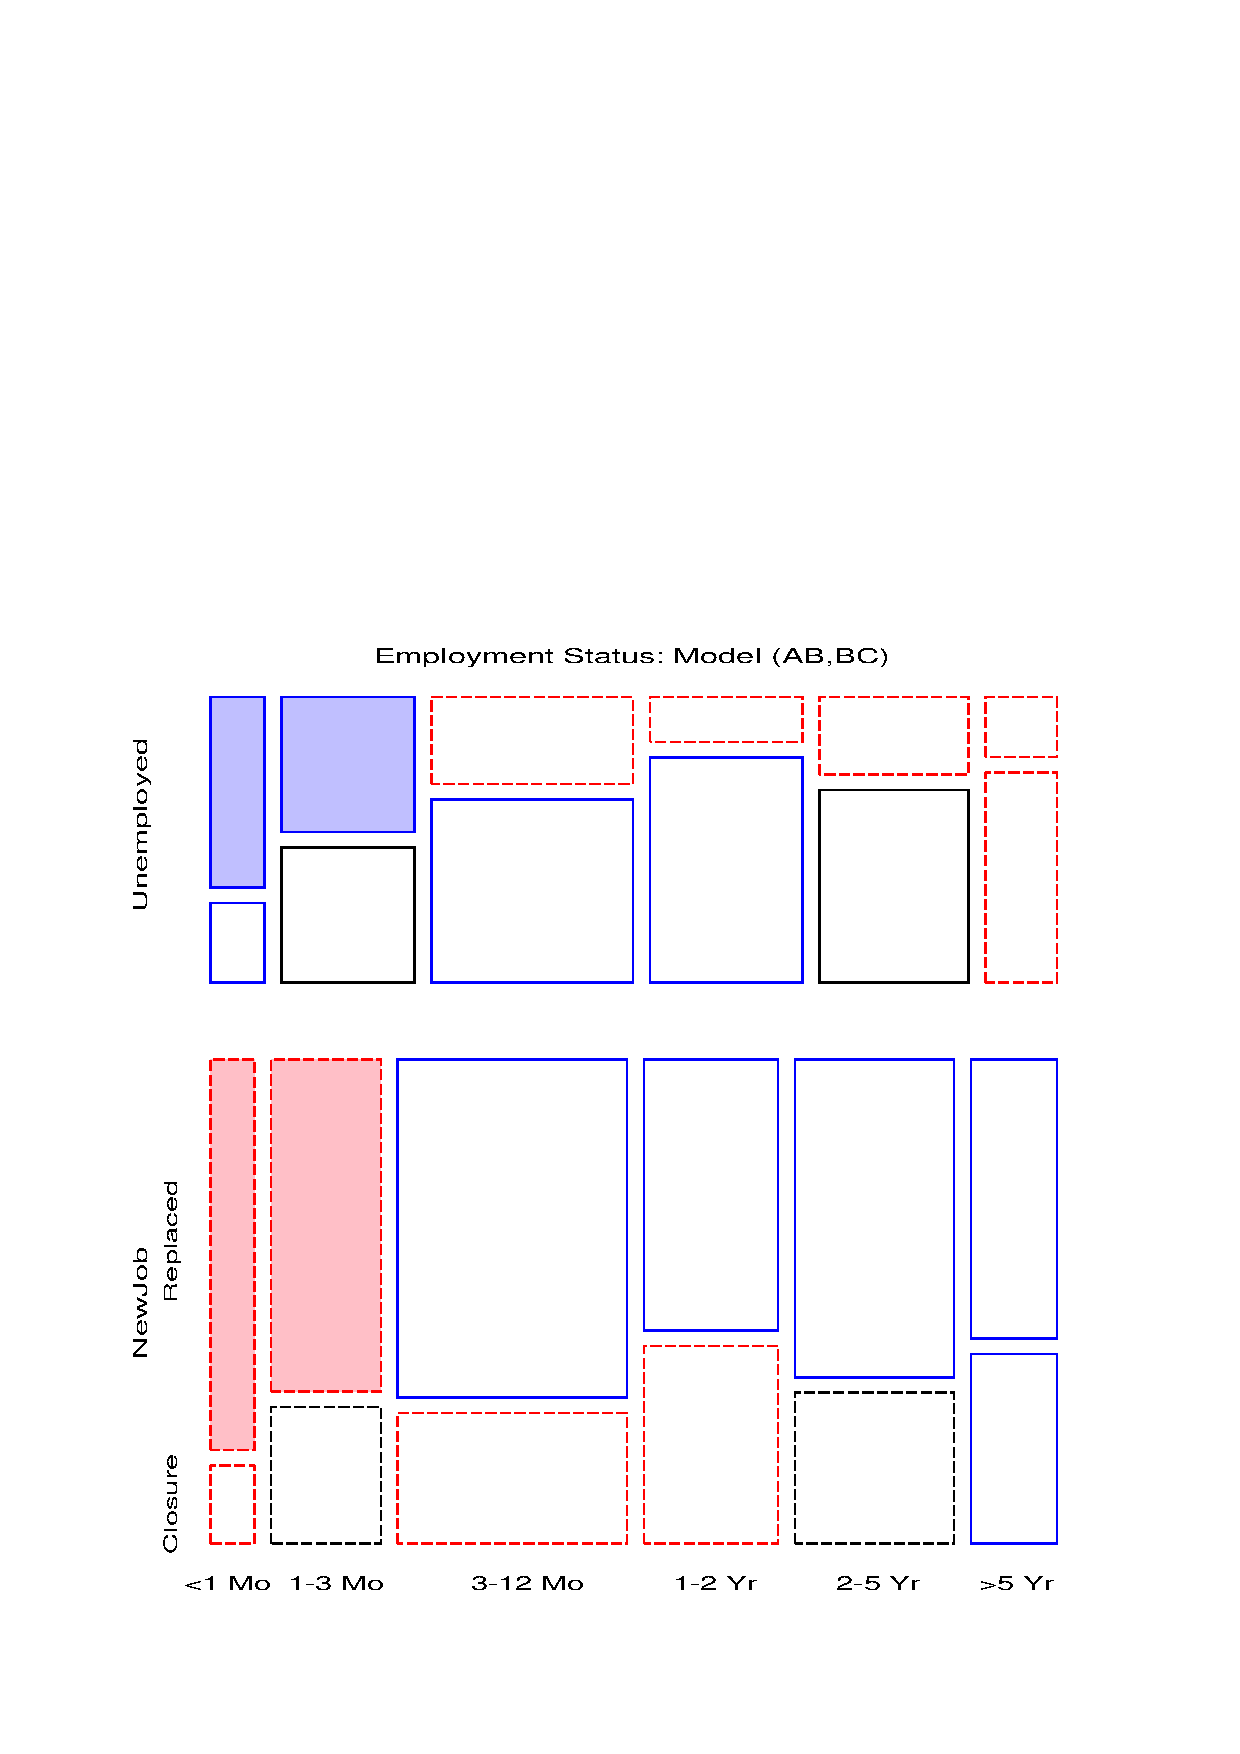
\includegraphics[scale=.6]{ch4/fig/mosaic143}
  \caption[Employment status data, conditional independence]{Mosaic display for the employment status data, fitting the model of
conditional independence, \LLM{AB,BC}, \(G^2 (10) = 24.63\)}
  \label{fig:mosaic143} 
\end{figure}

%% one figure
\begin{figure}[htb]
  \centering
  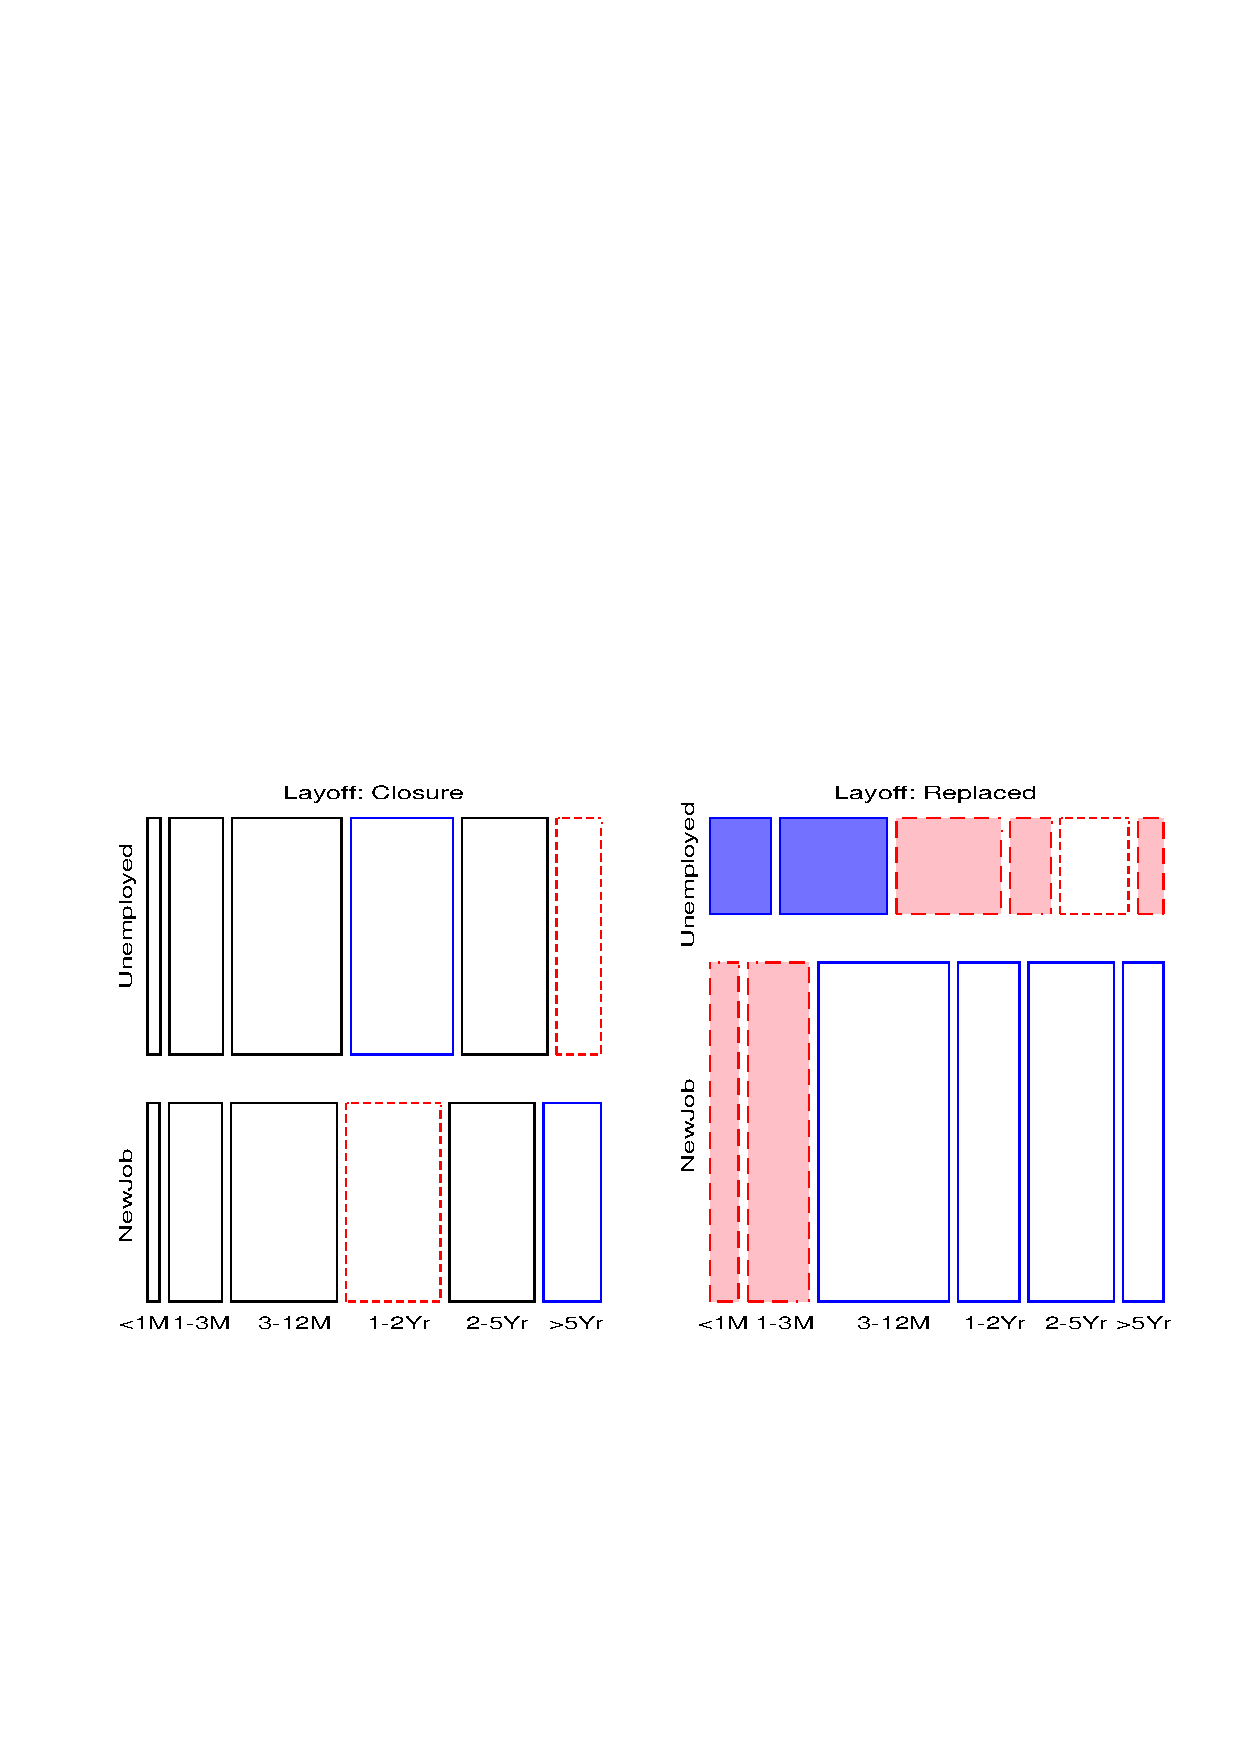
\includegraphics[width=\linewidth,clip]{ch4/fig/employp}
  \caption[Partial mosaic plots for employment status data]{Partial mosaic plots for employment status data. Each panel fits a model of independence
  between employment status and length of previous job.}
  \label{fig:employp}
\end{figure}

In order to test this notion, we fit the model $[A] \, [C]$
(employment status independent of length)
to each subtable separately for the causes of layoff.
The mosaic displays for closure and for replacement are
shown in \figref{fig:employp}.
These are produced with the \macro{MOSAICS} as shown below.
Using \texttt{BY=Layoff} gives a separate two-way plot for
each cause of layoff.
%% input: /Users/friendly/sasuser/mosaics/employp.sas
%% last modified: 18-Jul-99 12:34
\begin{listing}
title 'Employment status data';
data employ;
   length employed $10;
   input length $ @;
   do layoff ='Closure ', 'Replaced';
      do employed = 'NewJob   ', 'Unemployed';
         input count @;
         output;
         end;
      end;
   input;
datalines;
<1M       8   10     40   24
1-3M     35   42     85   42
3-12M    70   86    181   41
1-2Yr    62   80     85   16
2-5Yr    56   67    118   27
>5Yr     38   35     56   10
;
%gdispla(OFF);
%mosaic(data=employ, vorder=Employed Length Layoff, sort=no, 
    by=Layoff, shade=1 2 4, split=H V, fuzz=0.1, htext=2);

%gdispla(ON);
%panels(rows=1, cols=2);
\end{listing}


The residuals are all quite small when the cause of layoff
is a closure, and the $G^2 (5) = 1.44$, indicating 
that the chances of getting a new job are independent
of length of employment in this case.
On the other hand, when the cause of layoff is a replacement
the $G^2 (5) = 23.19$
and the residuals are large, particularly for the first
two length-of-employment categories.
These two subfigures represent the partition of the $G^2$
in \eqref{eq:partial1}.
\medskip
\begin{center}
\begin{tabular}{lrr}
 \hline
Model   &      df  &  \(G^2\) \\
 \hline
 $A \perp C \given B_1$  &  5   &   1.44 \\
 $A \perp C \given B_2$  &  5   &  23.19 \\
 \hline
 $A \perp C \given B$    &  10  &  24.63 \\
\end{tabular}
\end{center}
The partial mosaic plots in \figref{fig:employp} show clearly that
there is no association between employment status and length of
job among workers laid off due to closure.
Among replaced workers, those who had been employed less than or
equal to three months are likely to remain unemployed, while those
with longer job tenure are more likely to have found a new job.
\end{Example}